\documentclass[12pt,twocolumn,twoside]{conference}   %%
\usepackage[german, english]{babel}                  %%
%%% Vorgaben %%%%%%%%%%%%%%%%%%%%%%%%%%%%%%%%%%%%%%%%%%


\title{Technique and procedures of business analytics}

\author{}

\begin{document}
\twocolumn[
  \begin{@twocolumnfalse}
  \maketitle\thispagestyle{firststyle}
    \begin{abstract}
    \vspace{8pt}
Bei Business Analytics handelt es sich um eine Art Werkzeug für den Bereich des Controllings in einem Unternehmen. Das Werkzeug soll zur Lösung zukünftiger Probleme, anhand vergangener Informationen, verwendet werden.
Dieses Paper handelt von diesen Business Analytics und dessen umfassenden Verfahren, Vorgehensweisen und Methoden. Zuerst wird darüber berichtet, was Business Analytics sind. Danach folgt eine Analyse, über eine mögliche, strukturierte Vorgehensweise bei Business Analytics und wie sie gestaltet werden kann. Anschließend wird über das Verfahren des sogenannten Knowledge Discovery in Databases (KDD) und dort speziell auf das Data Mining eingegangen. Zu guter Letzt werden Predictive Analytics und die zu empfehlenden methodischen und architektonischen Vorgehensweisen.
    \end{abstract}
    \vspace{16pt}
  \end{@twocolumnfalse}
]

\section{Business Analytics}
\subsection{Business Analytics - Einleitung}
Früher war es die Aufgabe eines sogenannten Controllers, mit den Zahlen zu jonglieren und so die wirtschaftlichen Zahlen eines Unternehmens zu prüfen und wiederzugeben. Heutzutage hat sich dies aber geändert. Der Aufgabenbereich eines Controllers ist in den letzten Jahrzehnten um einiges komplexer und technisch versierter geworden. Heutzutage ist einer der Hauptaufgaben eines Controllers, sogenannte "Business Analytics" anzuwenden, um das Unternehmen wirtschaftlich zu halten, sodass es immer noch auf dem Markt vertreten sein kann. Doch was genau sind diese Business Analytics?
Um einen besseren Einblick über die Business Analytics zu geben, werden zunächst folgende Fragen beantwortet: 

\begin{enumerate}
\item Was genau sind Business Analytics?
\item Wie ist der generelle Ablauf bei Business Analytics?
\item Wieso nutzt man Business Analytics?
\item Wieso werden Business Analytics so viel Aufmerksamkeit gewidmet?
\item Anwendungsfelder von Business Analytics
\item Was ist bei Business Analytics zu beachten?
\item Welche Analyse Tools bezüglich Business Analytic gibt es?
\end{enumerate}

\subsection{Was sind Business Analytics?}
Unter Business Analytics versteht man das Verfahren der Erforschung und der Evaluation  historischer Daten für die zukünftige Orientierung des Unternehmens.  Wie bereits oben beschrieben, werden sie hauptsächlich als eine Art Werkzeug des Controllers gesehen. Mithilfe der Business Analytics werden, historische Daten des Unternehmens oder auch die Daten des Unternehmensumfeldes genutzt, um Entscheidungen treffen zu können, was für einen Kurs das Unternehmen einlenken sollte, um auch zukünftig wirtschaftlich agieren zu können. Es wichtig zu verstehen, dass es sich bei Business Analytics um einen andauernden Prozess handelt, welcher in mehrere Phasen unterteilt ist. Dieser wird in dem folgenden Unterbereich behandelt.

\subsection{Business Analytics - Genereller Ablauf}

\begin{figure}[H]
\centering
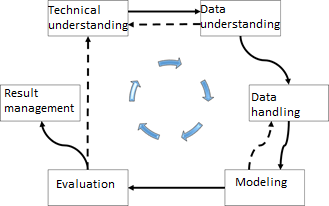
\includegraphics[width=8cm]{Abbildungen/Business_Analytics_Process.png}
\caption{Business Analytics Process}\label{visina8}
\end{figure}

Dieser oben dargestellte, andauernde Prozess kann in etwa so interpretiert werden, dass der Controller ein gewisses fachliches Verständnis benötigt, um ein Gespür für die relevanten Daten zu entwickeln. Diese können und sollten nach Änderung der Marktgegebenheiten, Änderungen interner bzw. externer Strukturen, oder gar von Zeit zu Zeit angepasst werden. Situationsabhängig werden nun die Daten, welche in die Analyse einzuspeisen sind, vorbereitet und Modelliert. Auch hier ist es möglich, dass die Daten, welche zur Modellierung der Analyse dienen, mehrmals angepasst werden müssen. Ist die Modellierung nun abgeschlossen, kommt es zur Evaluierung der aus der Analyse gewonnenen Ergebnisse. Nun kann es sein, dass diese Ergebnisse nicht hilfreich sind, oder zu wenig Aussagekraft für die aktuelle Analyse bieten. Falls dies der Fall sein sollte, wird das fachliche Verständnis erneut aufbereitet und vertieft. Es ist auch möglich, dass das fachliche Verständnis von den Ergebnissen der Evaluation profitiert und anhand dessen eine neu ausgereifte Analyse gestartet werden kann. Falls die ursprüngliche Analyse jedoch gewünschte bzw. erhoffte Resultate liefert, werden diese nun verteilt bzw. weitergegeben, sodass das Unternehmen die nächsten Schritte zur Optimierung der Wirtschaftlichkeit einleiten kann. Zu guter Letzt wird der beschriebene Analyseprozess auf einen anderen, bedürftigen Bereich des Unternehmens angewendet, um die Wirtschaftlichkeit dieses Bereichs zu optimieren.

\subsection{Wieso nutzt man Business Analytics?}
Die Frage, weshalb man Business Analytics nutzt, ist leider nicht mit einem Satz zu beantworten. Man nutzt Business Analytics, um große Datenmengen, oder auch "Big Data", zu analysieren, beurteilen und zum Schluss auch noch zu bewerten. Ein sehr großer Vorteil an dem Verfahren ist es, dass man selbst uneinheitliche Daten, optimal strukturieren und auswerten kann. Dank dieser Auswertung ist es zum Beispiel möglich, das Konsumverhalten der Käufer zu interpretieren und analysieren und im besten Fall herausfindet, dass man wenn man die Produktionskosten des meistverkauften Produkts, durch intensive Forschung, senken kann und somit mehr Gewinn generiert. Wie bereits beschrieben, handelt es sich hier nur um einen Anwendungsfall. Zusammenfassend lässt sich also behaupten, dass durch den Einsatz von Business Analytics, und die dadurch generierte - zum Beispiel - Marktforschung, positiv auf die Unternehmen auswirkt, die es verwenden.

\subsection{Wieso werden Business Analytics so viel Aufmerksamkeit gewidmet?}
Das Konzept der Business Analytics, welches auf dem Prinzip der Business Intelligence beruht, ist definitiv kein neues. Die ersten Ansätze der Business Intelligence wurden bereits Ende der 50iger Jahre veröffentlicht (siehe Wikipedia) und befassten sich mit der kontinuierlichen Datenerfassung innerhalb eines Unternehmens. Warum also, wird diesem Thema auch heutzutage noch so viel Beachtung geschenkt? Zum Einen, weil sich der Grundgedanke von Business Intelligence zu Business Analytics geändert hat. Es sollen nun also nicht mehr einfach die Daten erfasst und verwaltet werden, vielmehr werden diese zusätzlich noch sach- und fachgerecht ausgewertet. Zum Anderen weil die heutige technische Stand viel mehr Möglichkeiten bietet. Es ist zum Beispiel theoretisch möglich, den oben geschilderten Ablauf der Business Analytics, vollständig durch eine Hardware-Software-Kombination durchzuführen. 

\subsection{Anwendungsfelder von Business Analytics}
Wenn ein Unternehmen sich dafür entschieden hat, Business Analytics als Punkt zur Optimierung wahrzunehmen, muss auf  die richtigen Methoden und Algorithmen geprüft werden. Des Weiteren muss geprüft werden, was für eine Art von Business Analytics System in dem Unternehmen brauchbar sein wird. Dafür unterteilen  Mehenna et al die Anwendungsfelder der Business Analytics in folgende 5 Bereiche ein:

\begin{itemize}
\item Analyse
\item Forecast
\item Optimierung
\item Simulation
\item Radar
\end{itemize}

Diese 5 genannten Anwendungsfelder erlauben dem Business Analytics System, falls diese Anwendungsfelder in zusammenwirken sollten, das vollständige Potenzial zu nutzen (vgl. Mehenna et al. 2016 S.51) 

\subsubsection{Anwendungsfeld - Analyse}
Grundlage aller Business Analytics Systeme ist es, eine Analyse auf vorhandene historische Daten zu fahren. Hierbei wird das Anwendungsfeld der Analyse als Prozess gesehen, welcher impliziert, dass aus den einzelnen strukturellen Eigenschaften der Daten, Erkenntnisse gewonnen werden. Was für eine Art von Big Data Analyseverfahren genutzt wird, ist von Ziel zu Ziel unterschiedlich. Die Analyseverfahren werden im späteren Verlauf des Papers weiter erläutert. Das Ziel des Anwendungsfeld der Analyse ist es, dass man Fragen beantworten kann. 

\begin{@twocolumnfalse}
\begin{figure}[H]
\centering
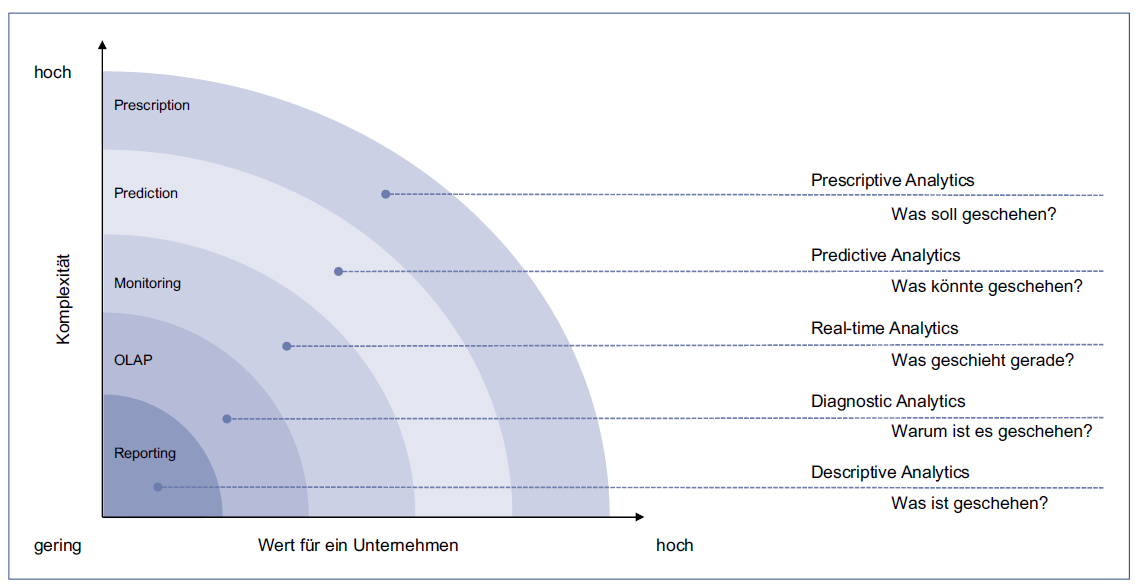
\includegraphics[width=20cm]{Abbildungen/Analysis.png}
\caption{Analysis Questions}\label{visina8}
\end{figure}
\end{@twocolumnfalse}

Wie Figure 2 entnommen werden kann, handelt es sich bei den Fragen die gestellt und beantwortet werden können, jeweils um eine andere Lösung des Business Analytic Systems. Im Rahmen des Anwendungsfeldes der Analyse, beläuft es sich jedoch ausschließlich um die sogenannten "Descriptive Analytics", die "Diagnostic Analytics" und die "Real-time Analytics". Die Descriptive Analytics kommen dem klassischen Reporting nach, wo im nachhinein analysiert wird, was, wann geschehen ist. Die Diagnostic Analytics entsprechen dem investigativem Ansatz. Hier wird sich vor allem gefragt, weshalb es zu einer entsprechenden Situation kommen konnte. Die letzte dargestellte Möglichkeit des Anwendungsfeldes der Analyse entspricht dem Prinzip der Real-time Analytics. Diese basieren aus einem Monitoring der sich im aktuellen Betrieb befindlichen System beziehungsweise Systemen. 

\subsubsection{Anwendungsfeld - Forecast}
Bei dem Forecasting handelt es sich um ein Werkzeug der Business Analytics, welches mithilfe von stochastischen Modellen, Maschinellem Lernen und Data-Mining-Ansätzen, effiziente Prognosen mit guten Ergebnissen gestalten lässt (vgl Mehanna, 2016). Auch hier gibt es noch einmal zusätzlich die Abgrenzung zu den sogenannten Digital Forecasts. Bei den Digital Forecasts können so eingesetzt werden, dass sie zum Beispiel am Ende, durch Kombination mehrerer dieser Digital Forecasts, die sogenannte EBITDA ,earnings before interest,taxes, depreciation and amortization, prognostizieren können. Dafür wurden in diesem Beispiel, folgende Forecasts miteinander kombiniert. Einmal die "Absatzprognosen auf Basis unstrukturierter Daten zu Trends". Dazukommend ein Forecast für das "Vollautomatisiertes Pricing". Anschließend noch eine "Frühzeitige Erkennung von Rohstoffpreisänderungen" und zu guter Letzt, noch eins für die "Optimierung der Lagerhaltung" (vgl. Mehanna et al. 2016). Das Ergebnis ist ein kontinuierlich lernender Umsatz-Forecast. 

\subsubsection{Anwendungsfeld - Optimierung}
Mithilfe der Forecasts beziehungsweise Digital Forecasts bekommt man nun Informationen über die zukünftige Entwicklung der Bereiche, auf denen das Forecasting anwegwendet wurde. Dies allein reicht natürlich nicht aus, um das  Unternehmen wirtschaftlicher agieren zu lassen. Ein weiterer, wichtiger Faktor, liegt im Bereich der Optimierung. Das Verfahren der Optimierung folgt dem Verfahren des Forecastings. Ein sehr gutes Beispiel der Optimierung ist das, der Optimierung des Warenbestands im Einzelhandels. Hier wird das System automatisch so angepasst, dass es, wenn ein Kunde einen Artikel ordert, automatisch mit der Bestandsmenge des Artikels im Lager verrechnet wird. Sobald ein vordefiniertes Minimum erreicht wird, wird dieser Artikel, im besten Fall, automatisch nachgeordert (vgl Mehanna et al. 2016). Das in diesem Beispiel erläuterte Modell, verringert sowohl die Kosten des Lagerbestandes des Unternehmens , als auch den Aufwand des Bestellens der neuen Ware. 'Modelle zur Identifikation neuer Ursache-Wirkungszusammenhänge können kontinuierlich weiterentwickelt werden und somit neue Erkenntnisse über Engpässe oder Ineffizienzen generieren. Auf der anderen Seite verkürzen automatisierte Analysen die Reaktionszeiten, ermöglichen „Hochfrequenzentscheidungen“ und führen laufend zu ad-hoc-Umsetzung von Optimierungsmaßnahmen.'\cite{PAPER2}. Der Fokus bei dem Verfahren der Optimierung liegt in der immer fortdauernden Optimierung des Gesamtsystems.

\subsubsection{Anwendungsfeld - Simulation}
Das Verfahren der Simulation, beschreibt die Simulation eines Unternehmens und die möglichen Entwicklungen in der Zukunft. 'Bereits heute werden verschiedene Szenarien einer möglichen Unternehmensentwicklung simuliert,
z. B. im Rahmen der Unternehmensplanung. Aktuell sind diese Simulationen allerdings durch hohen manuellen Aufwand und personellen Einsatz geprägt. Zudem wird kurzfristig nur sehr bedingt auf Änderungen in den Szenarien reagiert. In der Folge werden Simulationen zur Unternehmenssteuerung oft auf ein Minimum reduziert und können so nicht ihren Mehrwert entfalten. Dadurch gehen potenziell hoch relevante Steuerungsinformationen verloren.' \cite{Mehanna et al. 2016}. Worauf Mehanna und weitere eingehen ist, dass die Simulationen oft nicht genügend Bedeutung, Aufmerksamkeit und Ressourcen jeglicher Art geboten werden. Wenn sie einmal richtig vollkommen konzipiert werden würden und mit allen, für die Simulation, relevanten Daten gespeist werden würden, können Simulationen genutzt werden, um betriebliche Entscheidungen zu unterstützen. Für diese Art von Simulation, gibt es treiberbasierte Modelle, wie etwa der Erlössteuerung. Das Ziel des Modells der Erlössteuerung ist es, dass die verfügbaren Ressourcen jeglicher Art den höchsten Umsatz generieren. Im besten Fall ist der Forecast der Business Analytics die Basis dieses Modells. Alle hierfür relevanten Daten, wie zum Beispiel die Kapazität, die Preise, die Last, die Betriebsdauer et cetera, werden nun in das Modell der Erlössteuerung geladen. Das Ergebnis dieser Simulation sind zum Beispiel, optimierte Preise zu bestimmten Verkaufszeitpunkten (vgl. Mehanna et al. 2016). Hierbei ist es zu beachten, dass es sich bei der Simulation um eine Art 'lernender Algorithmus' handelt und dieser im besten Fall auch mit den tatsächlichen Werten gespeist werden sollte, damit diese in den kommenden Simulationen berücksichtigt werden. 

\subsubsection{Anwendungsfeld - Radar}
Unter dem Verfahren des Radars versteht man die andauernde Beobachtung und Analyse des Marktsegements in welchem sich das Unternehmen bewegt. Hier passt der Begriff Competitive Intelligence ins Spiel. Bei Competitive Intelligence werden Prozesse und Technologien einer Aufklärung des Marktes und ihrer zugehörigen Bestandteile, wie Patente, Kunden, Zuliefere, Wettbewerber et cetera, zusammengefasst (vgl. Mehanna et al. 2016). 
Die Grundlage für brauchbare Daten, welche ins Radar eingespeist werden können, dienen unter anderem Social Media Kanäle und allgemein alles was unter "Open Data" verstanden werden kann. Zu den Open Data gehören öffentliche Seiten sowie Foren und Webseiten verschiedener Unternehmen des gleichen Marktsegments. Diese Informationen werden über semantische Analysen analysiert. Dazu gehören Verfahren wie Natural Language Processing oder Text Mining. Des Weiteren sollten in das Verfahren des Radars alle relevanten Informationen beziehungsweise Erkenntnisse bezogen werden. Diese können einem Unternehmen dabei unterstützen, die eigene Marke Wettbewerbsfähiger zu machen, da man auch äußere Merkmale, wie die Wahrnehmung der eigenen Marke von einem Kunden, auswerten kann. Dank des Radars können heutzutage mehr Ressourcen in Innovationen gesteckt werden, was den aktuellen Wachstum an Produktvielfalt erklärt.

\subsubsection{Anwendungsfelder - Resümee}
Wie bereits erwähnt, handelt es sich bei den Business Analytics um einen erweiterten methodisch-technologischen Werkzeugkasten für den Bereich des Controllings. Die 5 Anwendungsfelder dienen der Orientierung und sollten definitiv nicht einzelnd betrachtet werden. In einem Unternehmen sollten, idealerweise, diese Anwendungsfelder Verknüpft werden und es wäre sogar sehr sinnvoll, ein System zu integrieren, welches eine Kombination aus allen fünf Anwendungsfeldern beinhaltet. Jedoch sollte zu beginn drauf geachtet werden, dass man die Anwendungsfeld-Systeme einzeln betrachtet und Erfahrungen mit ihnen sammelt, bevor man ein weiteres Anwendungsfeld-System integriert. 

\subsection{Was ist bei Business Analytics zu beachten?}
Bislang wurde in diesem Paper ausschließlich positiv von Business Analytics beschrieben. Wie kommt es dann, dass nicht jedes Unternehmen mit Business Analytics arbeitet? Einer der Gründe ist, dass die Investition in die Technologie selbst, relativ kostspielig ist und noch lange nicht alle Probleme löst. Wichtig ist es auch, dass die Anwender dazu in der lage sein müssen, die Probleme eingrenzen können und darauf dann ihre Analysen fahren. Nur derjenige, welcher im Vorhinein die richtigen Daten zur Analyse gibt, wird eventuell auf brauchbare Ergebnisse kommen. Des Weiteren ist es nicht nur relevant, welche Daten, der Analyse zur Verfügung gestellt werden, sondern auch mit welchem Algorithmus diese verarbeitet werden. Zusätzlich kommt der Stil der Visualisierung der Ergebnisse hinzu. Solange diese nicht entsprechend sinnvoll dargestellt werden, bringen einen die effektivsten Algorithmen und die besten Daten nichts. Zu guter Letzt liegt es jedoch immer an der endgültigen Interpretation der zuständigen Instanz. Wie sich hieraus schlussfolgern lässt, gibt es bei den Business Analytics auch eine beachtliche Menge an Risiken. Wie sollte man Business Analytics also verwenden? Carsten Felden hat es in seinem Blog wie folgt erläutert: 'Zunächst einmal ist bei einer Einführung von Business Analytics der Mehrwert für das Unternehmen zu bestimmen, da der erworbene Nutzen den Aufwand rechtfertigen muss. Eine weitere Facette ist die zu Grunde liegende projektorientierte und prozessuale Betrachtung. Das projektorientierte Charakteristikum entsteht daraus, dass es beispielsweise in der Natur von Data Mining-Ansätzen liegt, kein Regelkreis zu sein. Für die jeweiligen wertstiftenden Aufgabenstellungen sind jeweils neu Daten zusammenzustellen, zielorientierte Analyseoptionen für die dann zu Grunde liegenden Daten zu evaluieren und auszuführen, um die Ergebnisse im täglichen Geschäftsbetrieb einsetzen zu können.' \cite{Beispiel1:2016} Wie dem Text von Carsten Felden entnommen werden kann, sollte zunächst betrachtet werden, ob das Anwendungsgebiet des Unternehmens überhaupt einen Nutzen für Business Analytics wiedergibt oder nicht. Anschließend ist es wichtig, dass das System dauerhaft mit sinnvollen Informationen versorgt wird bzw. versorgt werden kann. Falls diese Punkte schon nicht dafür sprechen sollten, sollte sich das Unternehmen   nicht für einen Lösungsansatz basierend auf Business Analytics entscheiden.

\subsection{Welche Analyse Tools bezüglich Business Analytic gibt es?}
Da es sich bei Business Analytics mehr um einen Ansatz, als um eine konkrete Lösung handelt, gibt es auch hier verschiedene Analyse Tools. Hier sind einige der Gängigsten:

\begin{itemize}
\item A/B Tests
\item Statistische bzw. quantitative Analyse
\item Data Mining
\item Predictive Analytics
\end{itemize}

Während die A/B Tests, statistische bzw. quantitative Analyse und dem Data Mining schon ziemlich genaue Ansätze sind um den zukünftigen Kurs eines Unternehmens zu planen, handelt es bei den Predictive Analytics wiederum um ein Teilgebiet der Business Analytics. In den folgenden Kapiteln werden das Data Mining und die Predictive Analytics dargestellt.

\section{Data Mining}
\subsection{Data Mining - Einleitung}
Im Zuge der Business Analytics, gibt es viele Verfahren bzw. Tools um große Datenmengen zu analysieren und später zu evaluieren. Es ist kein großes Problem, Daten zu evaluieren, welche sich nur in den einzelnen Werten ändern. Was jedoch, wenn die Daten einen ungleichmäßigen Aufbau haben? Für den eben angesprochenen Fall, der sogenannten heterogenen Daten, gibt es das Verfahren des Data Minings. 

\subsection{Data Mining - KDD Prozess}
Im Grunde genommen ist das Data Mining ein Teilschritt, und zwar der, der Datenanalyse, des Knowledge Discovery in Databases-Prozesses. 'Ziel des KDD ist die Erkennung bislang unbekannter fachlicher Zusammenhänge aus vorhandenen, meist großen Datenbeständen. In Abgrenzung zum Data-Mining umfasst KDD als Gesamtprozess auch die Vorbereitung der Daten sowie die Bewertung der Resultate.' \cite{Beispiel2:2016}

\begin{figure}[H]
\centering
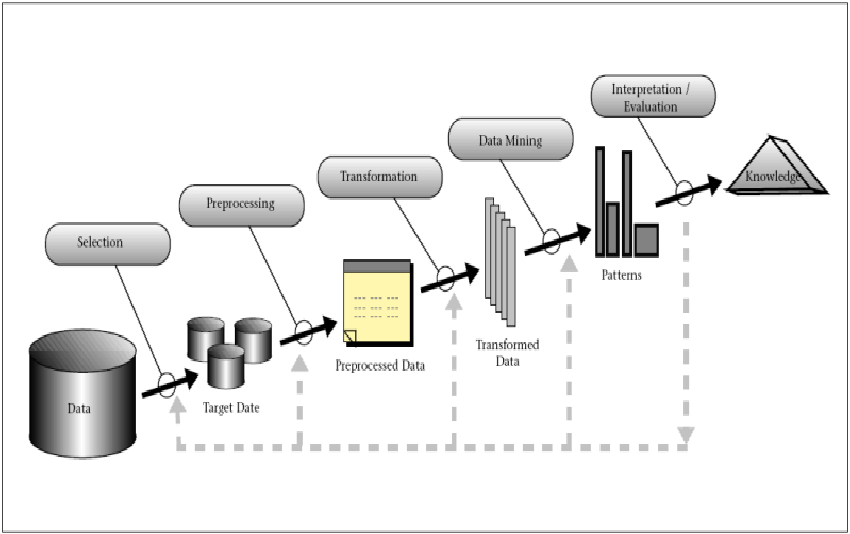
\includegraphics[width=8cm]{Abbildungen/KDD.png}
\caption{KDD Process}\label{visina8}
\end{figure}

Wie Figure 3 entnommen werden kann, besteht der KDD Prozess aus mehreren Teilschritten. Der erste Schritt, der Schritt der Selection, besteht daraus, dass zuerst das man aus dem Sammelsurium der zur Verfügung stehenden Daten, jene herauspickt, welche eine Bedeutung für die zu fahrende Analyse haben könnten. Anschließend werden diese preprocessed, damit Datenfehler entfernt und korrigiert werden. Nun folgt der Prozess der Datenreduktion, in dem die Daten auf den zu verarbeitenden Dateninhalt reduziert werden. Danach folgt der Schritt des Data-Minings, in welchem die eigentliche Datenanalyse gefahren wird. Das Ergebnis dieser Analyse wird in verschiedene, vorher ausgewählte Pattern geschoben und zu guter Letzt werden diese dann vom Nutzer evaluiert beziehungsweise interpretiert.

\subsection{Data Mining - Anwendungsverfahren}
Die Verfahren, in welche eine Data-Mining-Anwendung arbeitet, unterscheidet sich von Unternehmen zu Unternehmen und selbst hier von Situation zu Situation. Im wesentlichen sind die typischen Verfahren in die folgenden unterteilt(8 im Dokument):

\begin{itemize}
\item Anomalie-Analyse
\item Clusteranalysen
\item Klassifikation
\item Assoziationsanalysen
\item Regressionsanalyse
\end{itemize}

\subsubsection{Anomalie-Analyse}
Bei der Anomalie-Analyse handelt es sich um eine Analyseart, in der ein Mittelwert gebildet wird und jeder Datensatz welcher sich zu sehr von diesem Mittelwert unterscheidet, wird als suspicious markiert. Es ist üblich, dass als suspicios markierte Datensätze, von einem User manuell, auf Richtigkeit, überprüft werden.

\subsubsection{Clusteranalysen}
Bei sogenannten Clusteranalysen werden die Datensätze in gewissen Häufungen innerhalb eines Datenraumes analysiert. Falls ein Datensatz nicht in ein Cluster passt, wird er, je nach Verfahrensart, wie bei der Anomalie-Analyse, als suspicious markiert. Auch hier werden als suspicious markierte Datensätze, von einem User auf Richtigkeit geprüft.

\subsubsection{Klassifikation von Daten}
Ähnlich wie bei den Clusteranalysen, werden bei der Kassifikation von Daten, die Datensätze in einen Datenraum analysiert und abgebildet. Anders als bei der Clusteranalyse, werden diese Räume jedoch vor dem Analyseverfahren vordefiniert. 

\subsubsection{Assoziationsanalysen}
Die Assoziationsanalysen suchen Normalität bzw. Regelfälle in den Datensätzen. Diese Ergebnisse könnten zum Beispiel angeben, welche Art von Objekten in irgendeiner Art und Weise in Relation zueinander stehen. 

\subsubsection{Regressionsanalysen}
Bei der Regressionsanalyse steht die Analyse der Zusammenhänge einzelner Daten eines Datensatzes im Vordergrund. Dies erlaubt dem Nutzer zu erkennen, ob die Art der Datensätze vollständig sind, oder ob sie um  irgendwelche relevanten Attribute ergänzt werden sollten.

\subsection{Data Mining - Schlussfolgerung}
Abschließend kann gesagt werden, dass Data Mining Anwendungen den Zweck verfolgen, nicht triviale Muster in größeren Datenmengen aufzudecken. Die anschließend daraus gewonnenen Modelle werden üblicherweise auf aktuelle/zukünftige Datenkonstellationen angewendet um somit Informationen aus der gefahrenen Analyse ziehen zu können.

\section{Predictive Analytics}
\subsection{Predictive Analytics - Einleitung}
Predictive Analytics sind ein Verfahren, bei welchem historische Daten verwendet und evaluiert werden, um zukünftige Ereignisse vorherzusagen. Wo es beim Verfahren der Knowledge Discovery in Databases darum geht, die Daten auszuwerten und anhand dieser Auswertung, die nächsten Schritte einzuleiten, geht es bei Predictive Analytics darum, mithilfe der Daten, Modelle zur Auswertung zu generieren (vgl. Baars et al. 2016). 

\subsection{Predictive Analytics - Methodische Aspekte}
Da bei Predictive Analytics, der Fokus auf der vorhersage zukünftiger Ereignisse liegt, gibt es auch ein paar methodische Anforderungen an das Verfahren. Zum einen kommt es drauf an, woher die Informationen, welche zur Analyse genutzt werden, stammen. Hierbei sollte drauf geachtet werden, dass ausschließlich vertrauenswürdige Informationen aus dem nahen Umfeld bzw. selbst gesammelte Daten/Informationen genutzt werden. Es ist ebenfalls wichtig, dass dem Endnutzer, welcher die Ergebnisse evaluiert, neben den Ergebnissen auch die Werte gezeigt werden. Andererseits ist es wichtig, dass die eingesetzten Methoden, welche die Analyse durchführen, das Marktumfeld beziehungsweise die Branche berücksichtigen. Einer der methodischen Besonderheiten ist es auch, dass das System sowohl aus Benutzersicht modelliert wird als auch Zusammenhänge und Restriktionen vordefiniert werden, sodass das System für den jeweiligen Anwendungsfall effektiv arbeiten kann (vgl. Dr. Baars 2016)

\subsection{Predictive Analytics - Architektonische Aspekte}
Bei einem Predictive Analytics System empfiehlt sich der Einsatz mehrerer Systeme, welche für die Analyse zuständig sind. Für diese Zwecke wäre es sinnvoll, wenn man ein vom Produktivsystem getrenntes System in Form einer Sandbox betreibt. Des Weiteren benötigt es hochwertige Daten um Modelle generieren zu können. Diese, für die Analyse und Modellgenerierung relevanten Daten, sollten sowohl Interner- als auch externer Natur sein. Für das Sandboxsystem empfiehlt es sich ebenfalls eine Reihe von Tools zur Verfügung stehen zu haben, zum Beispiel Data Mining Tools sowie Datenmanipulations- und Datenintegrations-Tools(vgl. Dr. Baars 2016). Die Kombination von all diesen technischen Aspekten dient dazu, ein Analyseablauf beobachten zu können und die daraus resultierenden Informationen beziehungsweise Erfahrungen mit ins Produktivsystem zu übernehmen. 

\section{Fazit}
Business Analytics und speziell, Knowledge Discovery in Database und Predictive Analytics sind Ansätze, die in jeder IT-Branche Anklang finden könnten, da die Digitalisierung der Unternehmenssteuerrung mit Big data und Business Analytics einen Paradigmenwechsel anstoßen könnte(vgl. PAPER 2). Dort macht es keinen Unterschied ob in einem normalen Einzelhandel, oder bei Banken eingesetzt wird. Jeder dieser Sektoren könnte unheimlich von einem korrekt umgesetzten Business Analytics System profitieren. Wieso wurde es dann noch nicht überall umgesetzt? Ein großes Stichwort, welches gegen Business Analytics spricht, sind Kosten. Die Kosten die entstehen, um ein vollständiges Business Analytics System mit allen Komponenten aufzusetzen sind immens hoch. Des Weiteren muss erst ein gewisses Maß an Zeit unter Beobachtung vergehen, damit das System zum Produktivsystem gehören kann. Der letzte und wichtigste Punkt ist aber immer noch, der des Controlling Personals. Es kommt am Ende nicht drauf an, wie das System umgesetzt wurde, falls das Personal, die Ergebnisse der Analyse "falsch" evaluiert bzw. interpretiert, kann es sein dass ein Unternehmen einen falschen Kurs eingeht und die Wirtschaftlichkeit des Unternehmens darunter leiden wird. Ein Weiteres Problem ist, dass die datengetriebene Steuerrung noch lange nicht ausgereift ist. Meiner Meinung nach ist das Thema zwar mit Vorsicht zu genießen, aber definitiv Wert, weiterhin unter Beobachtung zu stehen. 
\newpage

\begin{thebibliography}{99}
	\bibitem{Beispiel1:2016}
	Beispiel1: http://www.enzyklopaedie-der-wirtschaftsinformatik.de/lexikon/daten-wissen/Business-Intelligence/Analytische-Informationssysteme--Methoden-der-/Business-Analytics 
	Aufgerufen am 23.06.2018 um 15:37 Uhr CEST
	\bibitem{PAPER2}
	Beispiel2: https://de.wikipedia.org/wiki/Knowledge-Discovery-in-Databases
	Aufgerufen am 19.06.2018 um 11:54 Uhr CEST
	\bibitem{ISO9075-1:2011}
	ISO/IEC 9075-1: Information technology
	Database languages -SQL- ,Part 1: Framework
	(SQL/Framework), 4. Auflage, ISO Copyright Office,
	Genf 2011
\end{thebibliography}

\end{document}
